\documentclass[]{article}
\usepackage[T1]{fontenc}
\usepackage{graphicx,hyperref}


\title{dynatop Manual}
\author{Paul Smith}
\date{2025-08-13}
\begin{document}
\maketitle




\tableofcontents
\section{Introduction}

This training course is split into two parts. Part 1 aims to:

\begin{itemize}
\item Provide an outline of Dynamic TOPMODEL as implemented in the \texttt{dynatop} and
\texttt{dynatopGIS} packages

\item Demonstrate the use the \texttt{dynatop} and
\texttt{dynatopGIS} packages with a hands on example

\item Give some suggestions as to the effective use of the \texttt{dynatop} and
\texttt{dynatopGIS} packages

\end{itemize}

Part 2 of the course is targeted at those that wish to extent or develop the packages and covers:

\begin{itemize}
\item Looking at the source code of \texttt{dynatop} by forking and cloning the software repository

\item Altering and building the source code

\end{itemize}

\subsection{Funding}

al;kkjsdf;lajkdf

\section{Prerequisites}

This is a course on hydrological modelling using a R software package.
Part 1 presumes that you have at least a basic knowledge of hydrology and
ideally some experience of R.
Part 2 requires a more detailed knowledge of R along with some knowledge of
the git version control system.

Useful primers for R can be found on multiple websites such as that of
\href{https://adv-r.hadley.nz/}{Hadley Wickham} or on
\href{https://cran.r-project.org/doc/manuals/r-release/R-intro.pdf}{CRAN} but
complete knowledge of their contents is not expected.

\subsection{Software}

\subsubsection{Part 1}

To make use of the examples on which Part 1 of the course is based requires

\paragraph{An installation of R 4.4.0 or above}

Installation instructions for R are available from
\href{https://cran.r-project.org/}{CRAN} for Linux, Windows and Mac.
Full details of the R version and packages used in building this version of
the training material can be found {here}.

\paragraph{A suitable text editor for altering the R scripts.}

While it is possible to complete the course using the built in R GUI's for
Windows and Mac it is recommended to install an editor with syntax
highlighting. Popular choices include the \href{https://www.rstudio.com/products/rstudio/download/\#download}{Rstudio
IDE}, VSCode
(Instructions
\href{https://www.r-bloggers.com/2021/01/setup-visual-studio-code-to-run-r-on-vscode-2021/}{here})
or Emacs with \href{https://ess.r-project.org/index.php?Section=home}{ESS} all of
which provide an integrated development environment.

\paragraph{Installed copies of \texttt{dynatop} and \texttt{dynatopGIS}}

These and there dependencies can be install in the standard way for R packages. At the R command
prompt type

\begin{verbatim}
install.packages('dynatop', repos =c('https://waternumbers.r-universe.dev','https://cloud.r-project.org'))
install.packages('dynatopGIS', repos = c('https://waternumbers.r-universe.dev', 'https://cloud.r-project.org'))
\end{verbatim}

\subsubsection{Part 2}

For completing Part 2 of the course which focuses on developing
dynatop further software is required.

\paragraph{An installation of the git version control system}

Details on installing git can be found on the software's \href{https://git-scm.com/downloads}{webpage}.
It is presumed that git is available from the command line.

\paragraph{An installation of the pandoc universal document converter}

Pandoc provides \href{https://pandoc.org/installing.html}{installation
instructions}.

\paragraph{Tools for building R packages which include source code}

The most efficient method of installing the tools required for building R
packages depends upon the platform:

\begin{itemize}
\item Windows: a single tool chain
\href{https://cran.r-project.org/bin/windows/Rtools/}{Rtools} is available.

\item Mac: requires Apple Xcode and GNU Fortran compiler. Details of the GNU
Fortran compiler version and other libraries that may be required are
provided on \href{https://mac.r-project.org/tools/}{CRAN}

\item Linux: ensure that gcc and gcc-c++ compilers are installed.

\end{itemize}

\paragraph{An account on \href{https://github.com/}{github}}

This is required to fork and alter the source code.

\subsection{Data and Scripts}

{Download} the data for the examples as a zip
file. Extracting this should give a directory ``eden\_data'' with four
subdirectories. In the code provided is is presumed that the working directory
of the R session is ``eden\_data''.

To save copying and pasting from the web pages the R code used in the
training course is {available}. These scripts
should be used alongside the course material.

\section{Dynamic TOPMODEL}

\begin{quote}
This a simplified, opinionated introduction. The original motivation for
Dynamic TOPMODEL can be found in  \href{https://doi.org/10.1002/hyp.252}{Beven \& Freer,
2001}

\end{quote}

\subsection{Motivation}

Dynamic TOPMODEL was originally conceived as \emph{``A new version of the rainfall-runoff model TOPMODEL
is described in which the assumption of a quasi-steady state saturated zone
configuration is replaced by a kinematic wave routing of subsurface flow\ldots{}''}
allowing for \emph{''\ldots{}the simulation of dynamically variable up-slope contributing
areas.''}

Revisiting the idea of TOPMODEL (which has done this mainly for hill slopes, but
see \href{https://doi.org/10.1002/hyp.1128}{Peters et al. 2003}) a
model is formulated by

\begin{itemize}
\item Classifying the catchment up into areas that respond in a hydrologically
similar manner

\item Determining the connectivity between each of the classes

\item Assigning each class to an appropriate Hydrological Representative Unit
(HRU), which solves the hydrological processes for a standardised unit

\end{itemize}

In the following these aspects are outlined with reference to the
implementation of Dynamic TOPMODEL in the \texttt{dynatop} and \texttt{dynatopGIS} packages.

\subsection{Classification and Connectivity}

\subsubsection{Classification (Part 1)}

The location of areas with a hydrological similar response is only every
going to be partially captured by spatial data. Past TOPMODEL and Dynamic
TOPMODEL applications have used classifications based on a topographic index
given by the logarithm of up-slope area divided by the local gradient. Using the
up-slope area gives some spatial ordering to the classes, but (as we will see
with the Eden data) it is not complete. Consider a
small catchment represented by a raster of spatial cells with the following topographic index classes

\begin{figure}
\protect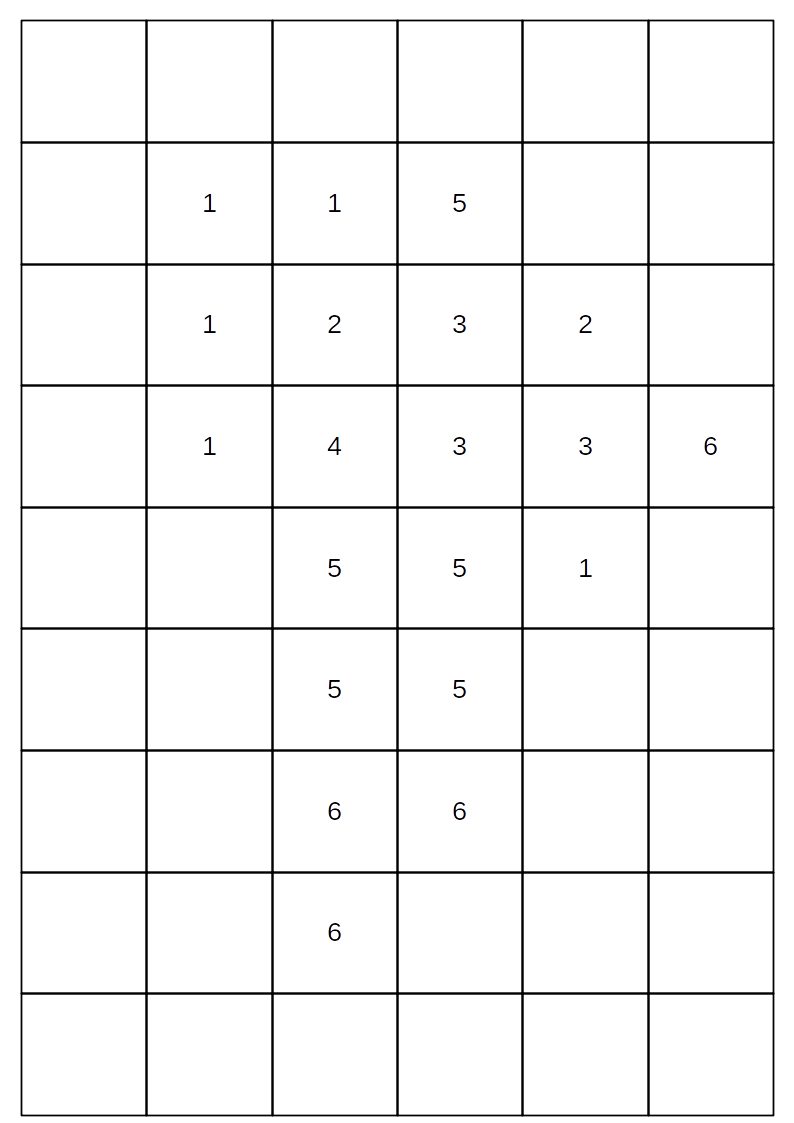
\includegraphics{./images/images/topo_class.png}

\caption{
\label{fig:topo_index} Map of topographic index classes
}
\end{figure}

Since land use could influence the evapotranspiration and infiltration
properties a second classification might be desirable. For the
small catchment the land use classes are shown below

\begin{figure}
\protect
\includegraphics{./images/images/landuse_class.png}

\caption{
\label{fig:land_use} Map of land use classes
}
\end{figure}

Combing these topographic index and land use classes gives one initial class
for each unique combination.

\subsubsection{Connectivity}

In keeping with earlier spatial analysis TOPMODEL and Dynamic TOPMODEL applications
connectivity (flow directions) is assumed to be determined by the surface
gradient with any down-slope region receiving flow. This gives a high degree of
connectivity between the spatial cells. If a river intercepts a cell it is
assumed that both the surface and subsurface flow direction change to follow
the river course.The following figure shows the
connectivity for the small catchment, with the river cells highlighted in blue.

\begin{figure}
\protect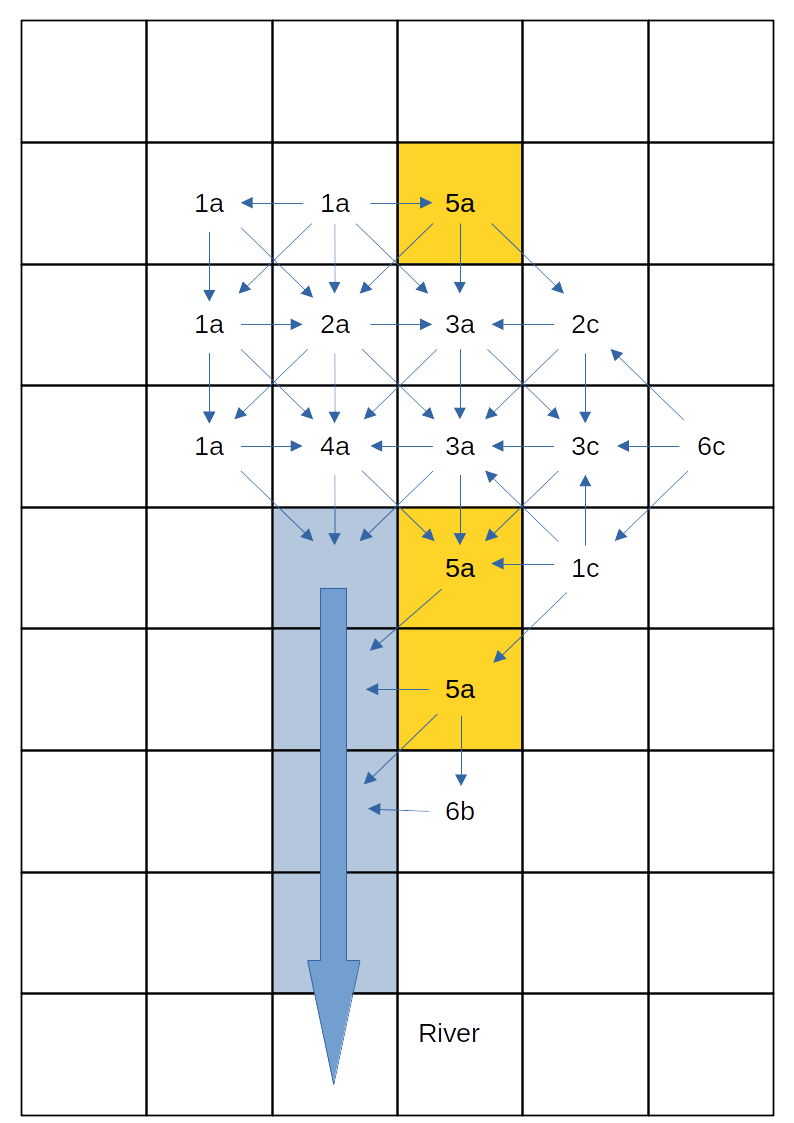
\includegraphics{./images/images/combined_class.png}

\caption{
\label{fig:combined_class} Map of combined topographic and land use classes along with connectivity
}
\end{figure}

\subsubsection{Classification (Part 2)}

Each class is represented by a single HRU, the inflows to which are
averaged from the inflows to all the spatial cells of that class.
Does this make sense for class 5a, which is both in the upper reaches
of the catchment but also adjacent to the river?

The \texttt{dynatop} author would argue not. To represent the spatial positioning the catchment can be banded using the connectivity - all cells
in a given band receive flows only from those in a higher band. For the small
catchment this looks like the following

\begin{figure}
\protect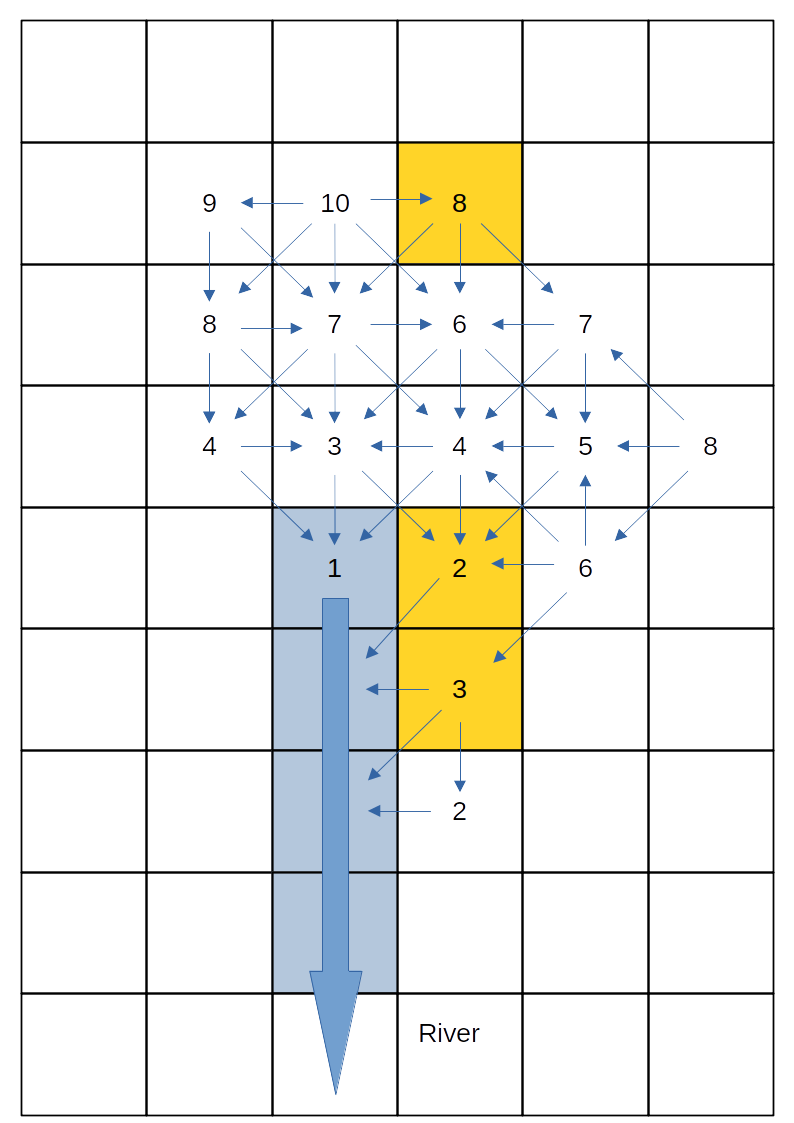
\includegraphics{./images/images/band_class.png}

\caption{
\label{fig:band} Map of the band classification
}
\end{figure}

Combing this into the classification gives

\begin{figure}
\protect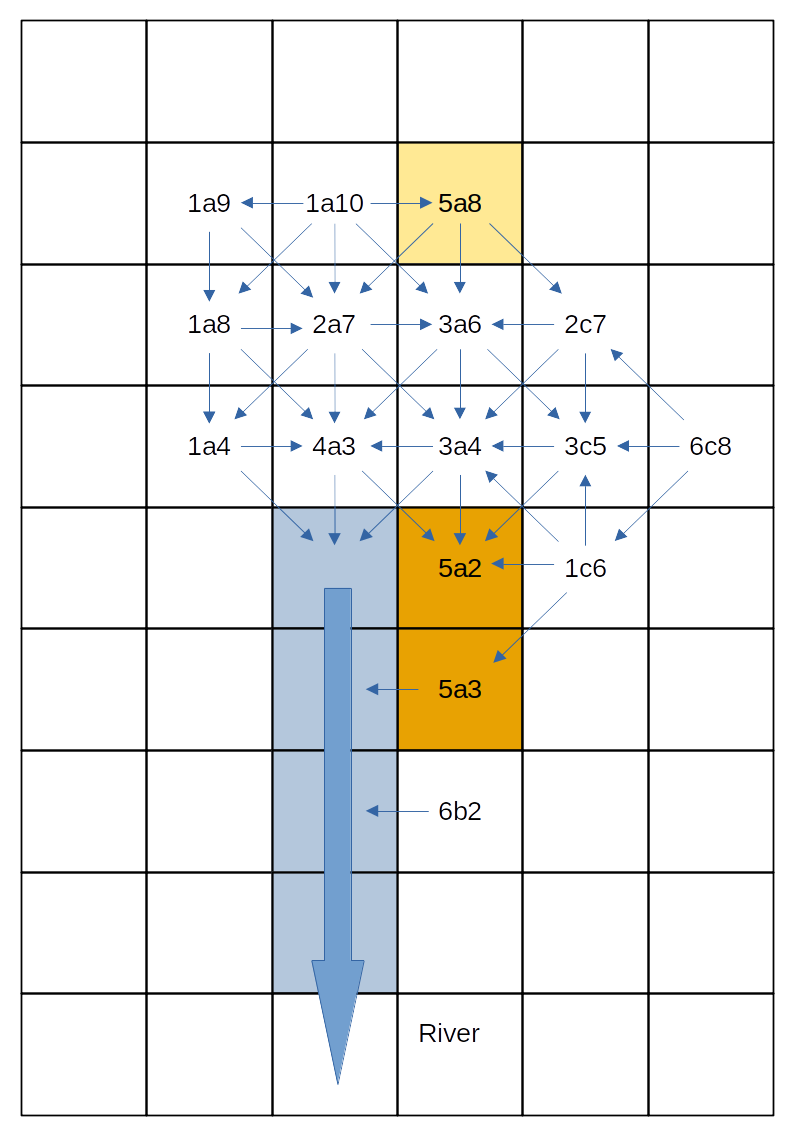
\includegraphics{./images/images/combined_class_with_band.png}

\caption{
\label{fig:combined_band} Map of the combined classification
}
\end{figure}

which further separates out the 5a class to the areas close to and further
from the river. This demonstrates the banding gives a further level of spatial refinement to the
classification while allowing a for simplification in the catchment representation.

Introducing the band into the classification has a further advantage. Solving
the HRUs starting with those in the highest band ensures that inflows at the
current time step are available for use in the numeric solution. This allow the use of
computation techniques that are more robust to the choice of solution time step.

\begin{quote}
The numeric scheme implemented in the \texttt{dynatop} package makes use of an
ordering so that the HRU inflows for the current time step are available. Although
other options could be used it is \textbf{strongly} recommended that the default
banding scheme is used.

\end{quote}

\subsection{Hydrological Response Units}

Each Hydrological Response Unit HRU represents a parameterised version
of a different part of the hydrological system. The representation of each HRU
is made up of the four zones:

\begin{itemize}
\item A \emph{Surface Zone} representing the movement of water on the surface

\item A \emph{Root Zone} which controls evapotranspiration, handles the precipitation
input and flux of water to the unsaturated zone

\item A \emph{Unsaturated Zone} which represented the water between the root zone and
the saturated subsurface

\item A \emph{Saturated Zone} representing the saturated subsurface

\end{itemize}

The following schematic shows the four zones and the fluxes between
them

\begin{figure}
\protect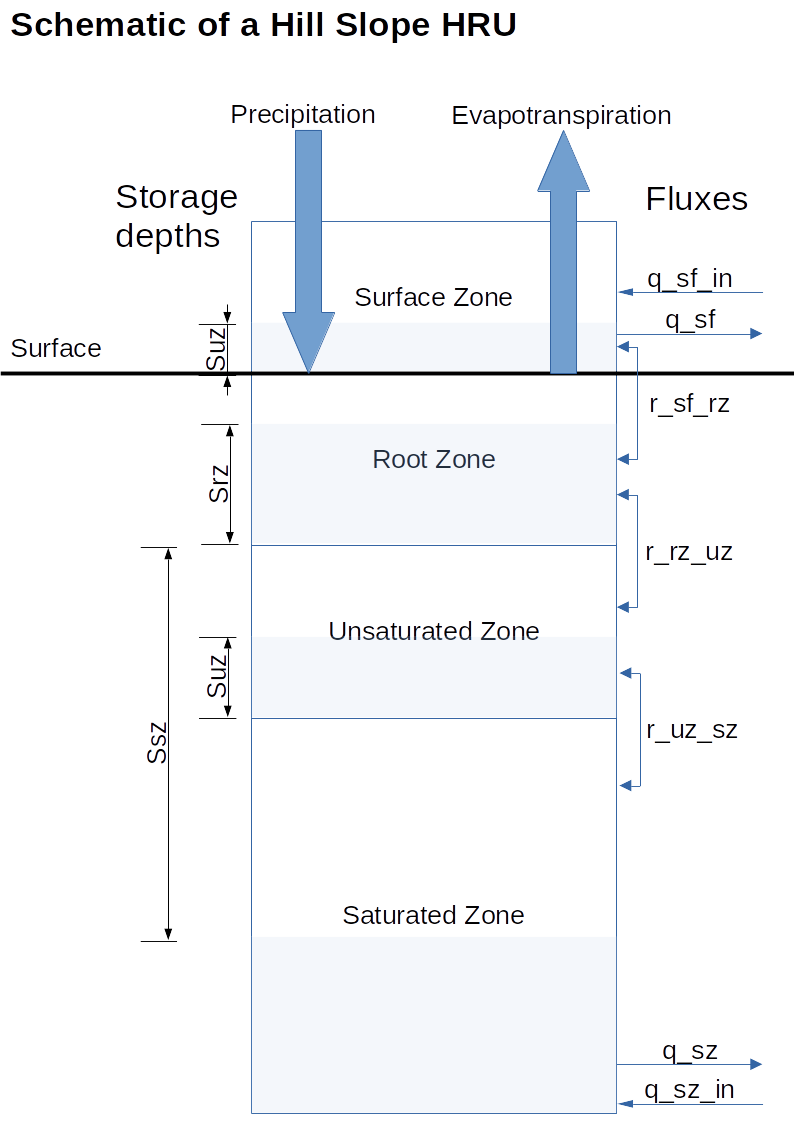
\includegraphics{./images/images/Hillslope_HRU.png}

\caption{
\label{fig:hru} Schematic of the Hill slope HRU
}
\end{figure}

As shown in the schematic fluxes are passed between the HRUs at two levels,
the surface and the saturated zones.

To allow for some flexibility in the dynamics of the HRU different
representations can be used for each zone. The governing equation and
numerical solution of these are given in a \href{https://waternumbers.github.io/dynatop/articles/HRU.html}{vignette of \texttt{dynatop}}. A few
key points are:

\begin{itemize}
\item The lateral flow from the Surface and Saturated Zones is computed using
Muskingham approximations.

\item Evapotranspiration is proportional to the percentage saturation of the Root
Zone

\item Flow from the root zone to the Unsaturated Zone can occur only when the Root
Zone is full

\item The Unsaturated Zone is represented by a tank whose time constant depends
upon the deficit of the Saturated Zone

\item The lateral flow from the Saturated Zone is controlled by the saturated
storage deficit through a transmissivity profile.

\end{itemize}

\section{dynatopGIS \& dynatop}

The following schematic outlines the stages resulting a working Dynamic
TOPMODEL for a catchment. It highlights where the \texttt{dynatopGIS} and \texttt{dynatop}
packages fit into this process.

\begin{figure}
\protect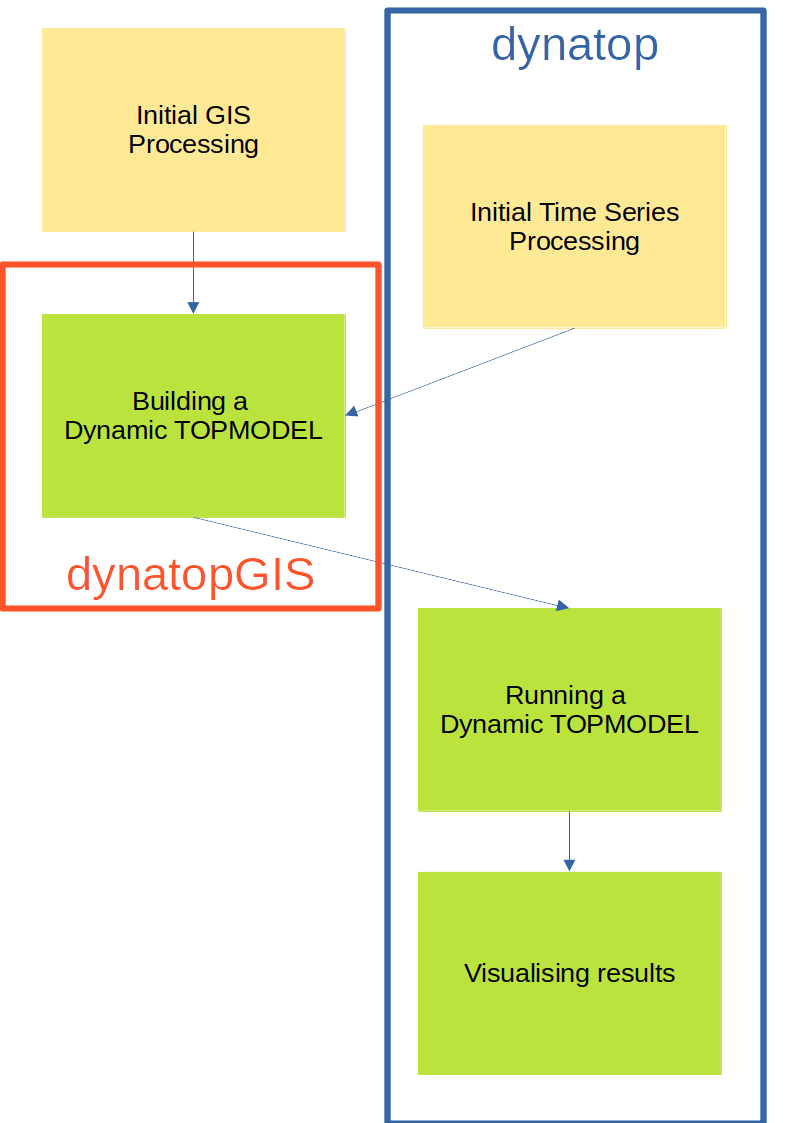
\includegraphics{./images/images/Build_Schematic.png}
construction''\}

\caption{
\label{fig:build_schematic} Schematic of a Dynamic TOPMODEL construction
}
\end{figure}

As we will see in the example the \href{https://waternumbers.github.io/dynatopGIS/index.html}{\texttt{dynatopGIS}} package can help

\begin{itemize}
\item Compute standard variables for classification (such as the topographic
index)

\item Compute the spatial ordering of the HRUs

\item Build classifications of the catchment

\item Construct models suitable for \texttt{dynatop}

\end{itemize}

The \href{https://waternumbers.github.io/dynatop/index.html}{\texttt{dynatop}} package allows simulation and visualisation of Dynamic TOPMODELs as well as
providing some helper for processing time series input data.
Although in this training presumes that model for \texttt{dynatop} are generated
using \texttt{dynatopGIS} this need not be the case so long as the inputs to
\texttt{dynatop} are of the correct format.

\section{Implementation notes}

The \texttt{dynatopGIS} and \texttt{dynatop} packages implement structured, object orientated, data
flows. The packages are written using the object orientated framework
provided by the \texttt{R6} package. This means that some aspects of working with the
objects may appear idiosyncratic for some R users. In this training these problems are largely obscured, except for the
call structure. However, before adapting the code, or doing more complex analysis
users should read about \texttt{R6} class objects (e.g. in the \texttt{R6} package vignettes
or in the Advanced R book). One particular gotcha is when copying an object. Using

\begin{verbatim}
my_new_object  <-  my_object
\end{verbatim}

creates a pointer, that is altering \texttt{my\_new\_object} also alters
\texttt{my\_object}. To create a new independent copy of \texttt{my\_object} use

\begin{verbatim}
my_new_object  <-  my_object$clone()
\end{verbatim}

\section{River Eden Example}

The first half of the training course is working through an example
application based on the Eden Catchment in Cumbria, UK (see Figure below). At the Sheepmount
gauging station downstream of Carlisle, which is the lowest
monitored point in the catchment, the total area is 2400 km\$\^{}2\$.

The River Eden and its main tributaries
including the Rivers Eamont, Irthing, Petteril and Caldew link a number of significant
areas for runoff generation which include the northern and eastern parts of the Lake
District; areas of the Northern Pennines and Kielder Forest. These areas are typified by
high annual rainfall totals and steep terrain. Moreover the confluences of two of
these main tributaries lie within the Carlisle urban area resulting in a complex situation
where significant inflows on any tributary may result in flooding.
In January 2005 Carlisle was flooded by an event with an estimated 0.0067 Annual
Exceedance Probability (AEP) at the Sheepmount Gauge (Clarke 2005; Day 2005).
Subsequently to this events in 2010, and particularly 2009, came close to over topping
the main flood defences. The significance of the 2005 flood, combined with a post
event survey of 263 water or wrack marks, has resulted in multiple inundation model
studies (Neal et al. 2009; Horritt et al. 2011; Fewtrell et al. 2011) and
modelling (Leedal et al. 2013, Smith et al. 2013).

\begin{figure}
\protect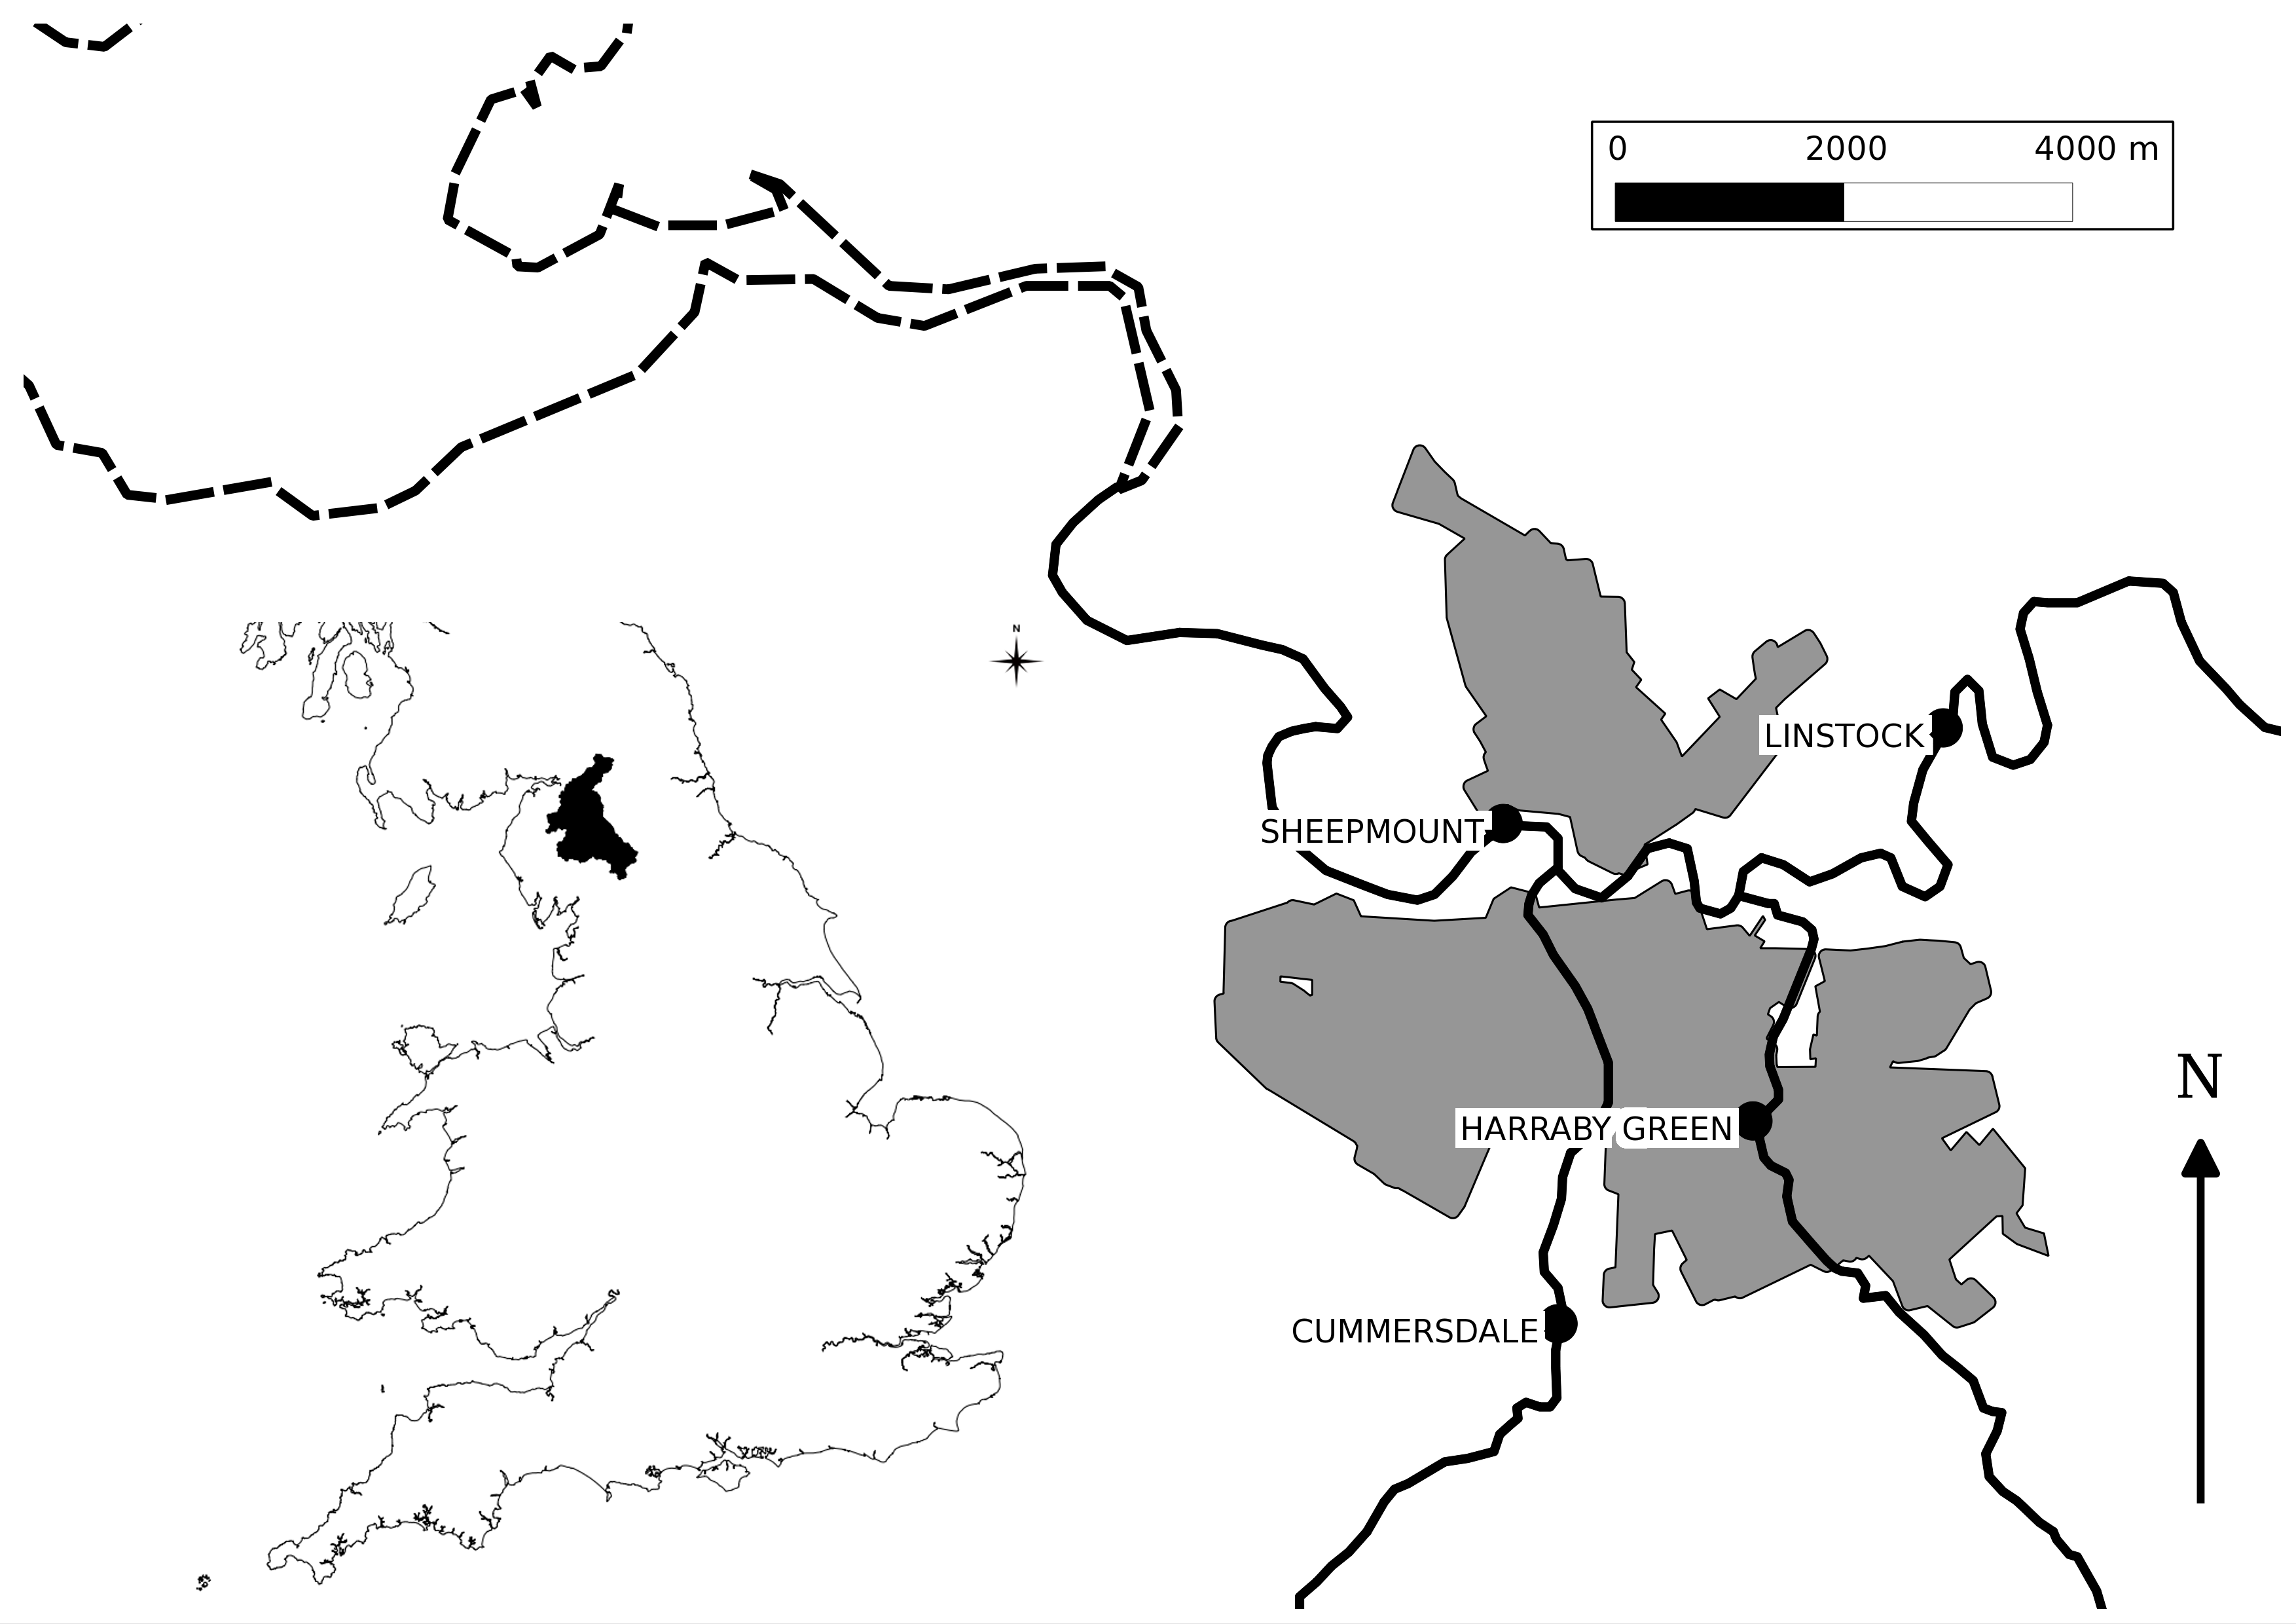
\includegraphics{./images/images/EdenMap.png}

\caption{
\label{fig:eden_map} Map of the River Eden Catchment
}
\end{figure}

\subsection{Available Data}

The directory ``eden\_data/unprocessed'' contains the starting data given in the
table below

\begin{table}
\begin{tabular}{lrl}
col 1 & col 2 & col 3 \\
a long row & and long row & a long row 1 \\
row 2 & row 2 & row 2 \\
\end{tabular}
\end{table}

\begin{table}
\caption{
\label{tab:simple} Available data
}

\begin{tabular}{lc}
File & Contents \\
Eden\_Flow.csv & Discharge data (m\$\^{}3\$/s) for the Sheepmount\textbackslash{} Gauge provided by the environment Agency \\
Eden\_Gauge\_Sites.csv & Locations of selected gauges in the Eden Catchment from the \href{https://nrfa.ceh.ac.uk/data/search}{NRFA} \\
Eden\_Catchment.* & Outline of the Study area and sub-catchments. Derived from gauge catchments in the \href{https://nrfa.ceh.ac.uk/data/search}{NRFA} \\
Eden\_Urban.* & Locations of urban areas as used in the 2011 census, from \href{https://data.gov.uk/dataset/15e3be7f-66ed-416c-b0f2-241e87668642/built-up-areas-december-2011-boundaries-v2}{data.gov.uk} \\
Eden\_Catchment.* & Outline of the Study area and sub-catchments. Derived from gauge catchments in the \href{https://nrfa.ceh.ac.uk/data/search}{NRFA} \\
Eden\_River\_Network.* & River Network within the catchment. Taken from \href{https://www.ordnancesurvey.co.uk/business-government/products/open-map-rivers}{OS Open Rivers} \\
Eden\_DEM.tif & Digital Elevation Model generated by aggregating \href{https://www.ordnancesurvey.co.uk/business-government/products/terrain-50}{OS Terrain 50} to 100m resolution \\
Eden\_Precip.nc & A time series of rainfall fields. Derived from the \href{https://gpm.nasa.gov/data/imerg}{GPM IMERG} final product by converting accrued rainfall in m \\
\end{tabular}
\end{table}



\end{document}
